\documentclass[11pt, oneside]{article}   	% use "amsart" instead of "article" for AMSLaTeX format
\usepackage{geometry}                		% See geometry.pdf to learn the layout options. There are lots.
\geometry{letterpaper}                   		% ... or a4paper or a5paper or ... 
%\geometry{landscape}                		% Activate for rotated page geometry
\usepackage[parfill]{parskip}    			% Activate to begin paragraphs with an empty line rather than an indent
\usepackage{graphicx}				% Use pdf, png, jpg, or eps§ with pdflatex; use eps in DVI mode
								% TeX will automatically convert eps --> pdf in pdflatex		
\usepackage{amssymb}
\usepackage{hyperref}
\usepackage{mathtools}
\usepackage{enumerate}
\usepackage{tikz}
\usepackage{algorithm}   
\usepackage{algpseudocode} 
\newcommand{\ck}[1]{\textcolor{cyan}{CK: #1}}
\newcommand{\jc}[1]{\textcolor{orange}{JC: #1}}
\newcommand{\hm}[1]{\textcolor{blue}{HM: #1}}

\title{Homework 5 \\ CSC 277 / 477 \\ End-to-end Deep Learning \\ Fall 2024}
\author{John Doe - \texttt{jdoe@ur.rochester.edu}}
\date{}					


\begin{document}

\maketitle

\begin{center}
    \textbf{Deadline:} See Blackboard    
\end{center}


\section*{Instructions}

Your homework solution must be typed and prepared in \LaTeX. It must be output to PDF format. To use \LaTeX, we suggest using \url{http://overleaf.com}, which is free.

Your submission must cite any references used (including articles, books, code, websites, and personal communications).  All solutions must be written in your own words, and you must program the algorithms yourself. \textbf{If you do work with others, you must list the people you worked with.} Submit your solutions as a PDF to Blackboard. 


Your programs must be written in Python. The relevant code should be in the PDF you turn in. If a problem involves programming, then the code should be shown as part of the solution. One easy way to do this in \LaTeX \, is to use the verbatim environment, i.e., \textbackslash begin\{verbatim\} YOUR CODE \textbackslash end\{verbatim\}.



%%%%%%%%%%%%%%%%%%%%%%%%%%%%%%%%%%%%%%%%%%%%%

\clearpage


\section*{Problem 1 - Out-of-Distribution Detection (11 Points)}
Out-of-distribution (OOD) detection refers to identifying data points that do not conform to the same distribution as the training data. In this context, a classifier needs to reject a novel input from classes unseen during training rather than assigning it an incorrect label. Two broad categories of methods have been developed to enable a model for OOD detection:
\begin{enumerate}
    \item \textbf{Inference Methods}: These techniques create an explicit acceptance score function to distinguish novel inputs from familiar ones based on the confidence or uncertainty measure associated with a model's predictions.
    \item \textbf{Regularization Methods}: Regularization approaches modify the feature representations of a model during training. The objective is to enhance the model's ability to discriminate between in-distribution and novel samples.
\end{enumerate}

\begin{figure}[h]
    \centering
    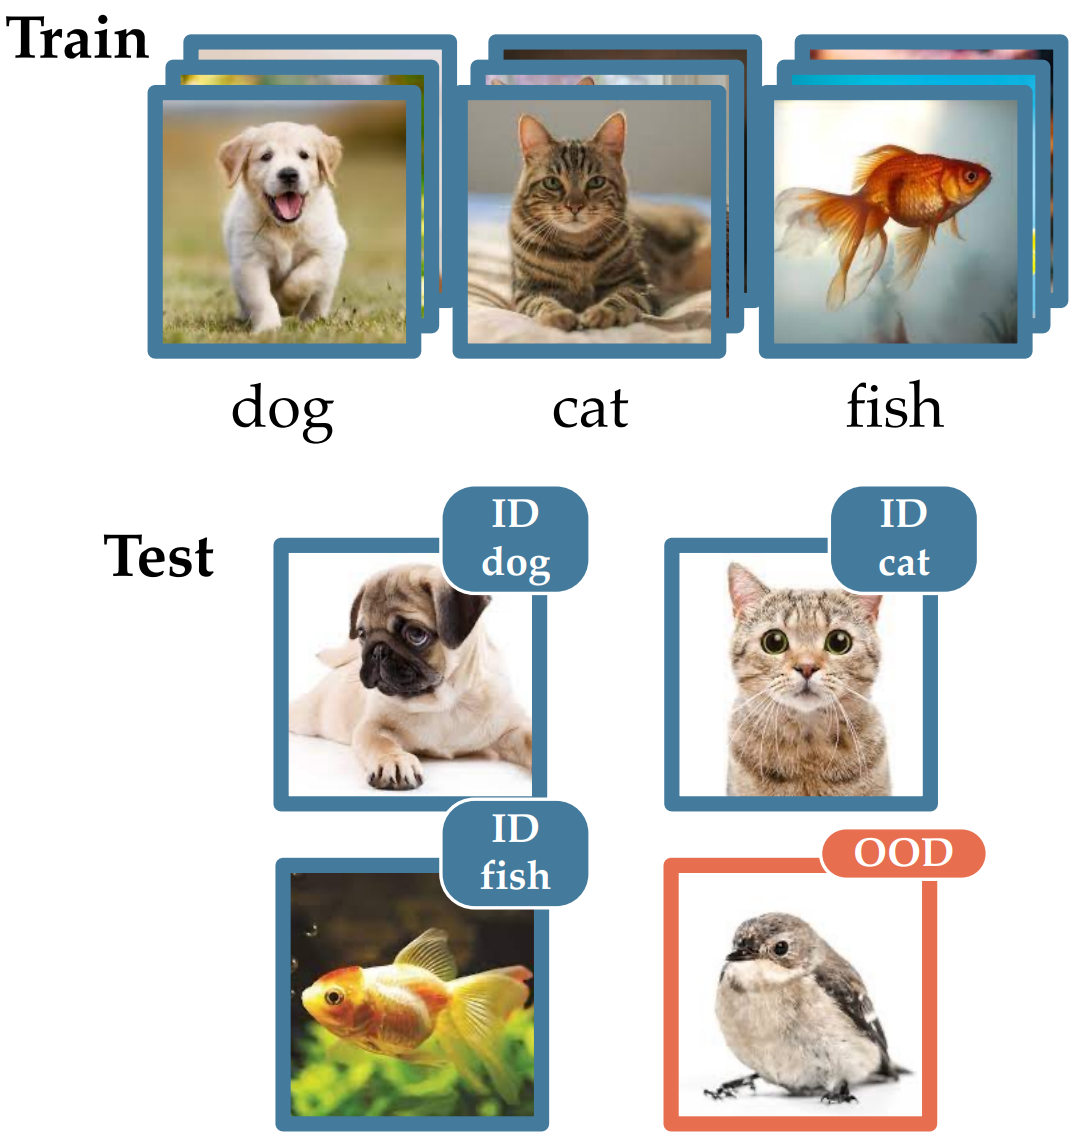
\includegraphics[width=0.4\textwidth]{images/ood.png}
    \caption{
    Illustration of \href{https://arxiv.org/pdf/2110.11334.pdf}{OOD task}. ID stands for in-distribution.
    }
    \label{fig:lora}
\end{figure}

In this problem, you will leverage the \href{https://github.com/kkirchheim/pytorch-ood}{pytorch-ood} package to explore various OOD detection methods, which not only implements commonly used methods but also provides readily available pre-trained models and datasets.
To get started with this problem, begin by following the package installation instructions and its dependencies as outlined in the provided guide. Please note that upgrading to the latest version of PyTorch may be necessary if you encounter any error messages during package usage.
\subsection*{Part 1: Inference Method}
\label{sec:part1}
\subsection*{Part 1.1: Maximum Softmax Probability Thresholding (6 Points)}
The Maximum Softmax Probability (MSP) Thresholding method represents a straightforward baseline approach for OOD detection. This method is designed to assess the confidence of a model's predictions by analyzing the final output of the model after applying the softmax activation function. The goal is to determine if a given input falls within the known classes or if it should be classified as an OOD instance.

Formally, the MSP score for a given input instance is defined as:

$$- \max_y \sigma_y(f(x) / T)$$

Where $\sigma$ is the softmax function, $T$ is the optimal temperature, and $\sigma_y$ indicates the $y^{th}$ value of the resulting probability vector. 

\textbf{Intuitive Understanding}: The intuition behind MSP Thresholding is that if the maximum softmax score, a heuristic measure for certainty, is low, the model is uncertain about the most likely class for a given input. This uncertainty implies that the input might not belong to the classes seen during training, making it a potential candidate for an OOD instance.

In this section, you will assess the performance of the MSP Thresholding baseline method on a pre-trained model using the CIFAR-10 training dataset. 
Follow the steps below to familiarize yourself with the usage of this package and learn how to perform OOD detection:
\begin{enumerate}
    \item Begin by following the quick start \href{https://github.com/kkirchheim/pytorch-ood#-quick-start}{guide}
    \begin{itemize}
        \item Load a WideResNet model pretrained on CIFAR-10 by setting the \texttt{pretrained} parameter to \texttt{cifar10-pt}.
        \item Prepare an MSP detector using the \texttt{detector.MaxSoftmax} class with the default temperature settings.
        \item Instantiate an \texttt{OODMetrics} class.
    \end{itemize}
    \item Define the Test Set for OOD Detection:
    \begin{itemize}
        \item Create a test set for OOD detection. This set combines the CIFAR-10 \href{https://pytorch.org/vision/main/generated/torchvision.datasets.CIFAR10.html#torchvision.datasets.CIFAR10}{\textbf{test set}}, with the \href{https://pytorch-ood.readthedocs.io/en/latest/data.html#lsunresize}{resized LSUN} dataset. For guidance on obtaining the evaluation transform for a pretrained model, refer to the code tutorial \href{https://pytorch-ood.readthedocs.io/en/latest/auto_examples/benchmarks/interface/cifar10_odin.html}{here}.
        \item You can use the \texttt{torch.utils.data.ConcatDataset} function to concatenate the two datasets effectively.
    \end{itemize}
    \item Perform OOD Detection on the Test Set:
    \begin{itemize}
        \item Follow the steps outlined in the quick start guide to perform OOD detection on the test set you've defined.
        \item Compute the metrics to evaluate the performance of your OOD detection method.
    \end{itemize}
    \item Generate an ROC Curve:
    \begin{itemize}
        \item While the \texttt{pytorch-ood} package may not provide a direct method for generating an ROC curve, you can access the necessary data for creating the curve within the Metric object. (Hint: refer to \href{https://github.com/kkirchheim/pytorch-ood/blob/dev/src/pytorch_ood/utils/metrics.py#L156-L157}{the implementation of the OODMetrics} for details on where the required data is stored.)
        \item Utilize libraries such as \texttt{sklearn} and \texttt{matplotlib} to create the ROC curve based on the retrieved data. 
        \item Save the data for usage in the next parts.
    \end{itemize}
\end{enumerate}

\textbf{Deliverable:}\\
\begin{enumerate}
    \item Provide the labels for data in the in-distribution and OOD datasets, along with the size of each dataset. Present your answer in a LaTeX table.
    \item Create a LaTeX table summarizing the logged metrics obtained from the \texttt{OODMetrics} class. Use up arrows ($\uparrow$) or down arrows ($\downarrow$) to indicate whether a particular metric is considered better when larger or smaller, respectively.
    \item Include the ROC curve you generated as part of your deliverable. 
    \item Briefly interpret the meaning of each metric in a few words. You may refer to Section 4.3 EVALUATION METRICS of \href{https://arxiv.org/pdf/1706.02690.pdf}{this paper}.
\end{enumerate}

\textbf{Answer:} \\

\subsection*{Part 1.2: ODIN (Out-of-DIstribution detector for Neural networks) (5 Points)}
ODIN is a technique designed to enhance the OOD detection capabilities of neural networks, which primarily focuses on modifying the input data during inference to increase the network's sensitivity to OOD samples. It includes two key steps:
\begin{enumerate}
    \item  \textbf{Perturbation}: ODIN perturbs the input data by adding a small, carefully chosen perturbation that makes OOD samples more distinguishable from in-distribution samples:
    $$\hat{x} = x - \epsilon \ \text{sign}(\nabla_x \mathcal{L}(f(x) / T, \hat{y}))$$
    where $\hat{y}$ is the predicted class of the network.
    \item \textbf{Temperature Scaling}: Similar to MSP, ODIN scales the logits of the model with a temperature parameter. 
\end{enumerate}

In this part, you will carry out OOD detection using ODIN. Follow the following steps:
\begin{enumerate}
    \item Begin by reading Section 3 of the \href{https://arxiv.org/pdf/1706.02690.pdf}{ODIN paper}. Understand the motivation behind input preprocessing in ODIN and how it relates to adversarial examples.
    \item Conduct an experiment by replacing the OOD detection method with ODIN, using its default hyperparameters.
    \item Repeat the experiment with ODIN, but this time use the hyperparameters specifically for the CIFAR-10 dataset, which is given \href{https://pytorch-ood.readthedocs.io/en/latest/auto_examples/benchmarks/interface/cifar10_odin.html}{here}.
    \item Create an ROC curve that includes the results from the \textbf{three} different settings you've experimented with so far (i.e., one for MSP, two for ODIN). Ensure that the labels and legends on the ROC curve are clear. Set the axis ranges according to Figure 1 in the \href{https://arxiv.org/pdf/1706.02690.pdf}{ODIN paper} to illustrate differences effectively.
    
\end{enumerate}


\textbf{Deliverables:}
\begin{enumerate}
    \item In a few words, explain how the perturbation process in ODIN relates to adversarial examples.
    \item Report the numerical metrics obtained from your ODIN experiments, including results for \textbf{both} the default and tuned hyperparameter settings. Give your result in a latex table. 
    \item Present the ROC curve containing the results of the three experiments. 
    \item Briefly compare the results of the ODIN experiments with those of the baseline method used earlier in your study. Consider the advantage(s) and disadvantage(s) of ODIN compared to the baseline.

\end{enumerate}

\textbf{Answer:} \\



\section*{Problem 2 - Continual Learning (6 Points)}
Continual learning focuses on training models that can progressively learn from data that becomes available over time. In an online learning (or streaming learning) setting, each data point is processed only once, and the data often exhibits non-independent and identically distributed (non-iid) characteristics. This poses a significant challenge for deep neural networks, which tend to suffer from \textbf{catastrophic forgetting}—the phenomenon where learning new information causes the model to forget previously acquired knowledge. Traditional fine-tuning methods typically fail in this scenario because they overwrite existing representations with new ones.

In this problem, you will compare a fine-tuning baseline with a simple yet effective continual learning algorithm, \textbf{Streaming Linear Discriminant Analysis} (SLDA), which has been developed to enable models to learn from new data while retaining past knowledge incrementally. Follow these steps:
\begin{enumerate}
    \item Read the \href{https://openaccess.thecvf.com/content_CVPRW_2020/papers/w15/Hayes_Lifelong_Machine_Learning_With_Deep_Streaming_Linear_Discriminant_Analysis_CVPRW_2020_paper.pdf}{paper}, specifically Section 3, and the SLDA implementation in \texttt{slda.py} to understand how SLDA works.
    \item Examine the attached code for this problem to understand the experimental setup. The dataset is split into 5 chunks, each containing a distinct set of classes. The model is trained on these chunks one after another and is evaluated on all learned chunks after each session.
    \item Execute the experiments by running \texttt{main.py} with and without SLDA. The performance will be printed out. Analyze the performance on the recently learned classes and the previously learned classes.
\end{enumerate}

\textbf{Deliverables:}
\begin{enumerate}
    \item What is the number of \textbf{trainable} parameters in the naive fine-tuning baseline? What is the number in Streaming LDA? Explain the differences by analyzing which parts of the model are trainable.
    \item Analyze the forgetting you observed in these two conditions (fine-tuning vs. SLDA) by tracking the performance on a specific chunk immediately after learning it and after learning subsequent tasks. Describe and interpret your findings.
    \item What happens when the data stream is iid? Present a table showing the average accuracy on the test set under these four conditions: Fine-tuning \textit{vs.} SLDA; iid \textit{vs.} non-iid data. Describe how data distribution introduces catastrophic forgetting. (Hint: 1. You can easily experiment with this condition by changing the \texttt{num\_split} parameter in \texttt{main.py}. 2. Assume each chunk of test data is of the same size, so you can compute the overall test accuracy by averaging the accuracies on each chunk.)
\end{enumerate}


\textbf{Answer:} \\

\end{document}   